\documentclass[t,11pt,british,english, top=1.0in]{beamer}
\usepackage{hyperref}
\usepackage{graphics}
\usepackage{amsmath}
\usepackage{amssymb}
\usepackage{natbib}
        %You can use the package \textbf{pgfpages} 
        %to arrange your slides for printing. This is also explained
        %in the \textbf{beamer} documentation.

\newcommand{\tensor}[1]{\overline{\overline{#1}}}
\newcommand{\tautens}{\tensor{\tau}}

\setbeamerfont{framesubtitle}{size=\normalsize}
\setbeamerfont{framesubtitle}{size=\normalsize}
%\setbeamertemplate{frametitle}[default][center]
%\setbeamersize{text margin left=6mm}

\usetheme{Madrid}
\usecolortheme{orchid}

%gets rid of bottom navigation bars
\setbeamertemplate{footline}[page number]{}
\setbeamertemplate{headline}{}

%gets rid of navigation symbols
\setbeamertemplate{navigation symbols}{}

\begin{document}
\title{Data Handling for Researchers\\\vspace*{5mm}\small Christian Jacobs, Matthew Piggott, Gerard Gorman, David Ham\\\vspace*{5mm}4 March 2014}
\author{} 
\date{} 

\frame{\titlepage} 

\frame{
   \frametitle{What is data?}
   \framesubtitle{Definition} 
   \begin{itemize}
    \item Data is a {\color{red}set of values} corresponding to one or more {\color{red}quantitative} or {\color{red}qualitative variables}.
    \vspace*{6mm}
    \item Examples:
      \begin{itemize}
        \item Sea levels measured every hour at a fixed location\vspace*{1mm}
        \item Speed of a car throughout time\vspace*{1mm}
        \item Metadata (= data that describes other data) for webpages\vspace*{1mm}
        \item Wind velocity at different locations in the UK
      \end{itemize}
     \vspace*{4mm}
    \item Data can come from {\color{red}existing sources}, may be {\color{red}derived} from several data sets, or a {\color{red}new independent data set} can be generated.
   \end{itemize}
}

\frame{
   \frametitle{What is data?}
   \framesubtitle{More examples} 
   Values of particle concentration in space:
   \begin{figure}[H]
      \centering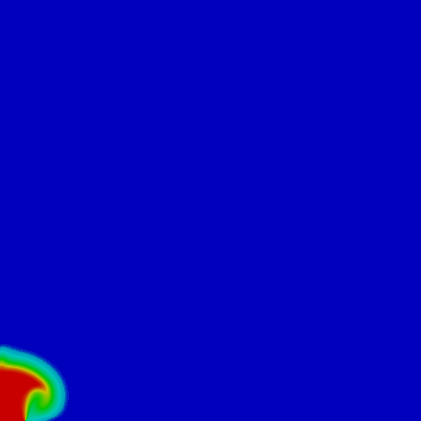
\includegraphics[width=0.32\columnwidth]{images/eruption_vfrac_10s.png}\hspace*{0.5mm}
      \centering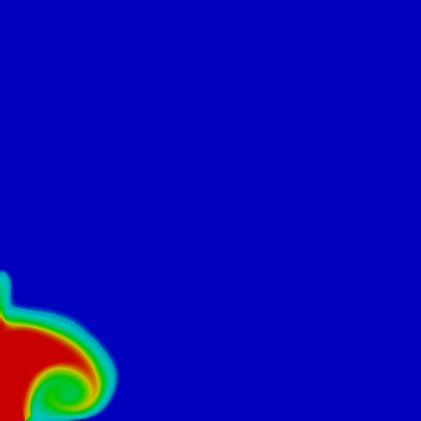
\includegraphics[width=0.32\columnwidth]{images/eruption_vfrac_30s.png}\hspace*{0.5mm}
      \centering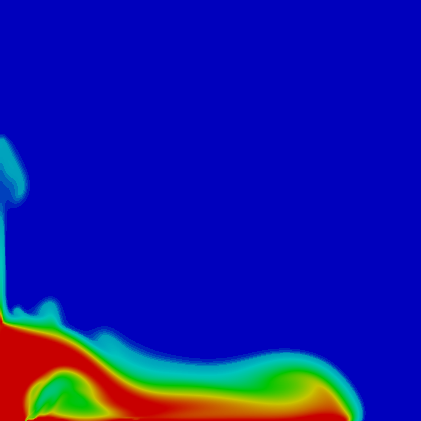
\includegraphics[width=0.32\columnwidth]{images/eruption_vfrac_70s.png}
      
      \centering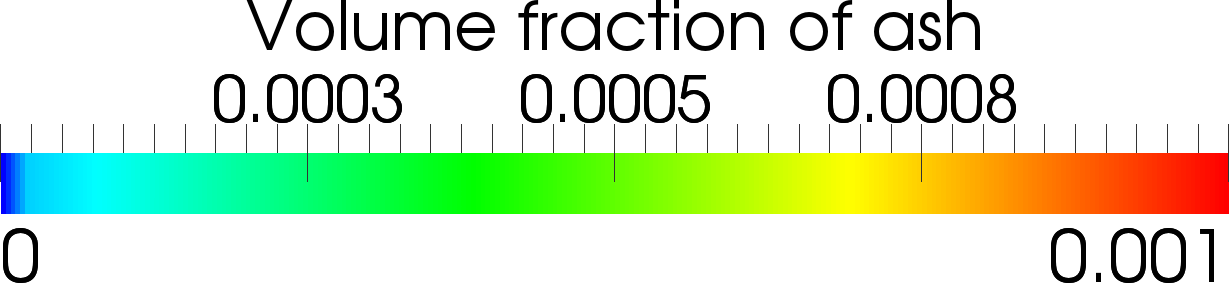
\includegraphics[width=0.3\columnwidth]{images/vfrac_legend.png}
   \end{figure}
}


\frame{
   \frametitle{What is data?}
   \framesubtitle{More examples} 
   Air density at various temperatures. Data from the Density page on Wikipedia.
   \begin{figure}[H]
      \centering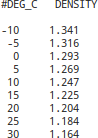
\includegraphics[width=0.25\columnwidth]{images/density.png}
   \end{figure}
}

\frame{
   \frametitle{What is data?}
   \framesubtitle{More examples} 
   Numerical solution error against grid spacing:
   \begin{figure}[H]
      \centering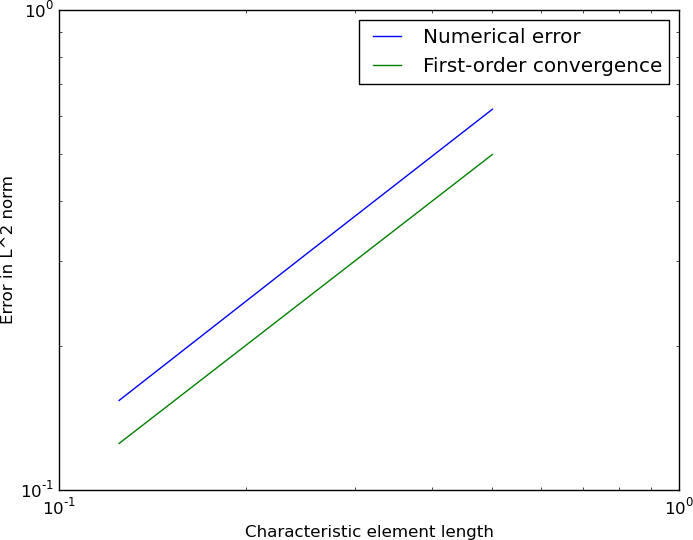
\includegraphics[width=0.7\columnwidth]{images/les_convergence.png}
   \end{figure}
}


\frame{
   \frametitle{Why is data important?}
   %\framesubtitle{Definition} 
   \begin{itemize}

    \item Allows {\color{red}new scientific discoveries} to be made.\vspace*{3mm}
    
    \item Journals and research councils are encouraging the {\color{red}sharing} of data to:
       \begin{itemize}
          \item promote research output,
          \item minimise the duplication of data,
          \item increase transparency and accountability, 
          \item allow fellow researchers to scrutinise and evaluate the data. 
       \end{itemize} \vspace*{3mm}
 
   \item The effective handling and management of all research data plays an important role in each of these processes. 
   
   \end{itemize}
}



\frame{
   \frametitle{Issues to consider}
   \framesubtitle{Data provenance} 
   \begin{itemize}
    \item {\color{red}Where} did the data originally come from? \vspace*{3mm}
    \item Can it be {\color{red}trusted}? (Is the author list available? Reputable journal?)\vspace*{3mm}
    \item Is it {\color{red}reproducible}?
   \end{itemize}
}

\frame{
   \frametitle{Issues to consider}
   \framesubtitle{Licensing} 
   \begin{itemize}
    \item {\color{red}Who} can use the data, and {\color{red}how}?\vspace*{3mm}
    \item Who owns the {\color{red}copyright}? Are you allowed to publish it or use it in your thesis?
    \vspace*{3mm}
    \item Any user licence? Creative Commons licences are becoming more popular and offer more freedom.\vspace*{3mm}
    \item Data produced when employed by a Government agency may be under Crown Copyright.
   \end{itemize}
}

\frame{
   \frametitle{Issues to consider}
   \framesubtitle{File formats} 
   \begin{itemize}
    \item Using {\color{red}standardised, open-source} file formats makes your data {\color{red}portable} and facilitates sharing of data by other researchers. \vspace*{3mm}
    \item Comma-Separated Value ({\color{red}CSV}): a commonly-used format for simple data sets. Values in a single row are separated by commas. CSV files can contain multiple rows, thereby forming a table. \vspace*{3mm}
    \item eXtensible Markup Language ({\color{red}XML}): each piece of data is encapsulated in a tag which annotates/describes it.
   \end{itemize}
}


\frame{
   \frametitle{Issues to consider}
   \framesubtitle{File formats -- CSV} 
   \begin{figure}[H]
      \centering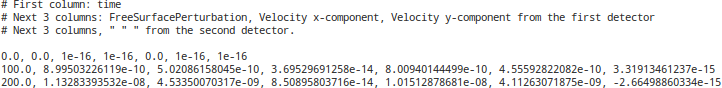
\includegraphics[width=1\columnwidth]{images/csv.png}
   \end{figure}
}

\frame{
   \frametitle{Issues to consider}
   \framesubtitle{File formats -- XML} 
   \begin{figure}[H]
      \centering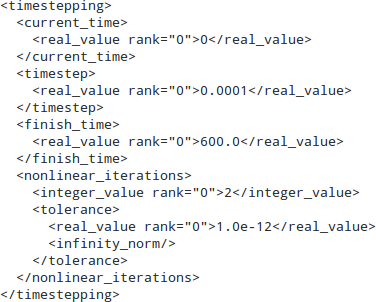
\includegraphics[width=0.7\columnwidth]{images/xml.png}
   \end{figure}
}

\frame{
   \frametitle{Issues to consider}
   \framesubtitle{Storage options}
   \begin{itemize}
    \item Optical media (CDs ~700 MB, DVDs ~4.7 GB, Blu-ray 25+ GB) and flash drives - for small files e.g. presentations, theses, papers.\vspace*{3mm}
    \item Magnetic media (hard drives) - for larger files (e.g. simulation output).\vspace*{3mm}
    \item Cloud services (e.g. Dropbox, Google Drive).\vspace*{3mm}
    \item Always maintain a good {\color{red}file hierarchy} and {\color{red}naming convention} when storing data files.
   \end{itemize}
}

\frame{
   \frametitle{Issues to consider}
   \framesubtitle{Backing up}
   \begin{itemize}
    \item \textbf{The importance of regularly backing up data cannot be stressed enough!}\vspace*{3mm}
    \item What if your hard drive failed right now? What if your computer was stolen?\vspace*{3mm}
    \item Storage space is reasonably cheap.\vspace*{3mm}
    \item Always keep {\color{red}several regular backups}, far apart from each other (not in the same building).\vspace*{3mm}
    \item Know the Imperial College data backup policy.
   \end{itemize}
}


\frame{
   \frametitle{Issues to consider}
   \framesubtitle{Encryption}
   \begin{itemize}
    \item Be aware of responsibilities to encrypt {\color{red}sensitive information}.\vspace*{3mm}
    \item Encrypting emails: Pretty Good Privacy (PGP) keys. \texttt{www.pgp.com}\vspace*{3mm}
    \item Encrypting hard drives: TrueCrypt (Windows, Linux, Mac OS), eCryptfs (Linux).
   \end{itemize}
}

\frame{
   \frametitle{Issues to consider}
   \framesubtitle{Big Data}
   \begin{itemize}
    \item {\color{red}Big Data} is one of the key challenges in data science.\vspace*{3mm}
    \item Involves data sets that are {\color{red}extremely large}, thereby creating additional difficulties when analysing them.\vspace*{3mm}
    \item Need novel and efficient tools to help tackle this issue.\vspace*{3mm}
    \item Data Science Institute at Imperial.
   \end{itemize}
}

\frame{
   \frametitle{Creating and manipulating data}
   \framesubtitle{Tools}
   \begin{itemize}
    \item Data sets are often {\color{red}merged}, {\color{red}manipulated}, and {\color{red}generated} using computer programs or scripts.\vspace*{3mm}
    \item Often written in MATLAB or Python.\vspace*{3mm}

   \end{itemize}
}

\frame{
   \frametitle{Creating and manipulating data}
   \framesubtitle{Quality assurance}
   \begin{itemize}
    \item Test programs for {\color{red}correctness} in order to have confidence in the results.\vspace*{3mm}
    \item Regression testing.\vspace*{3mm}
    \item Programs can break even without changes to the source code.\vspace*{3mm}
    \item The data itself should also be tested using {\color{red}verification} and {\color{red}validation} techniques.
   \end{itemize}
}

\frame{
   \frametitle{Creating and manipulating data}
   \framesubtitle{Quality assurance -- Buildbot}
   Buildbot: An automated testing framework.
   \begin{figure}[H]
      \centering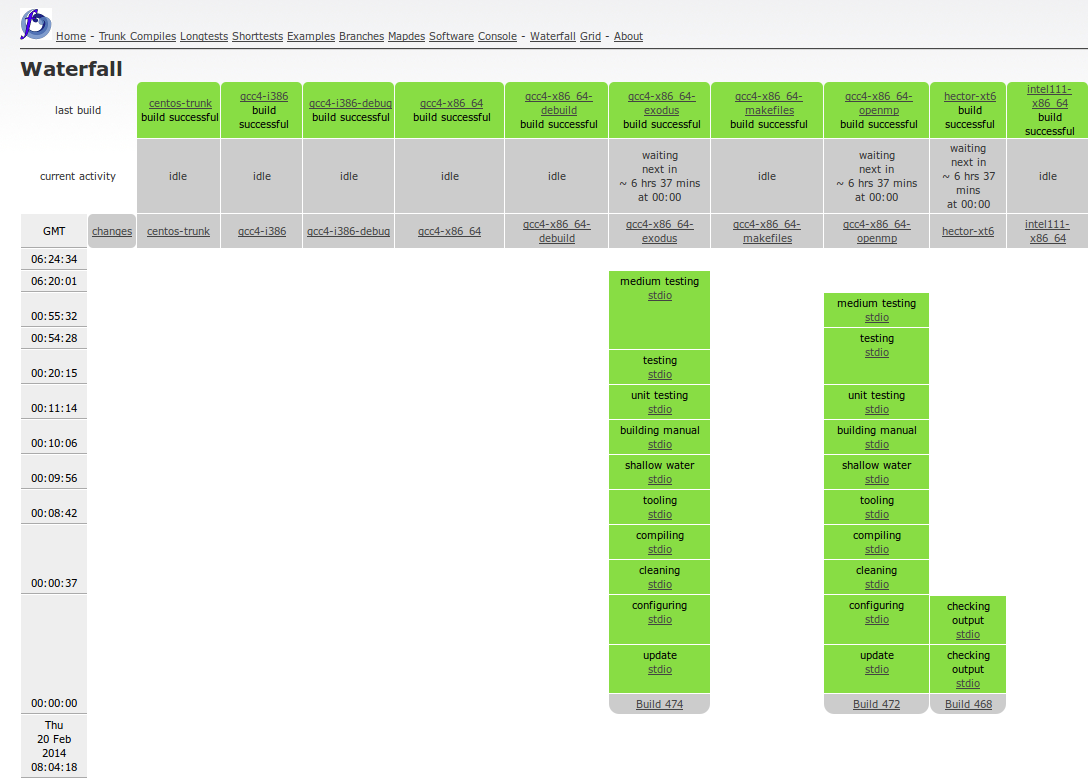
\includegraphics[width=1\columnwidth]{images/buildbot.png}
   \end{figure}
}

\frame{
   \frametitle{Creating and manipulating data}
   \framesubtitle{Commenting and documenting}
   \begin{itemize}
    \item Always {\color{red}comment} and {\color{red}document} your code to help yourself and others to understand how to use it.\vspace*{3mm}
    \item Use {\color{red}metadata} to document the name of the author, the date the data was created, any terms of use, etc.
   \end{itemize}
}

\frame{
   \frametitle{Creating and manipulating data}
   \framesubtitle{Version control systems}
   \begin{itemize}
    \item Used to keep track of changes to data, and the programs used to generate data.\vspace*{3mm}
    \item Facilitates team development.\vspace*{3mm}
    \item \texttt{git-scm.com} contains excellent documentation on the Git version control system.\vspace*{3mm}
    \item Some services such as GitHub (\texttt{www.github.com}) and Bitbucket (\texttt{www.bitbucket.org}) offer free Git-based repositories.
   \end{itemize}
}

\frame{
   \frametitle{Creating and manipulating data}
   \framesubtitle{Exercise 1}
   \begin{itemize}
    \item Let's work our way through a set of Git exercises created by GitHub: \texttt{http://try.github.io}\vspace*{7mm}
    \item Initialise a verson-controlled repository using \texttt{git init}\vspace*{3mm}
    \item Add files to the repository using \texttt{git add <file\_name\_here>}\vspace*{3mm}
    \item Remove files from the repository using \texttt{git rm <file\_name\_here>}\vspace*{3mm}
    \item Commit any changes using \texttt{git commit -a}
   \end{itemize}
}

\frame{
   \frametitle{Creating and manipulating data}
   \framesubtitle{Exercise 2}
   \begin{itemize}
    \item Bitbucket offers unlimited free {\color{red}private} repositories.
    \item Set up an account at \texttt{www.bitbucket.org}.\vspace*{3mm}
    \item More about the exercise to come.......
   \end{itemize}
}

\end{document}
